\documentclass[11pt]{amsart}
\usepackage[T1]{fontenc}
\usepackage{lmodern,microtype,amsmath,amssymb,mathtools,booktabs,array,tikz,pgfplots}
\usepackage[margin=1.05in]{geometry}
\usepackage[hidelinks]{hyperref}
\usetikzlibrary{arrows.meta,positioning}
\pgfplotsset{compat=1.18}
\raggedbottom
\setlength{\emergencystretch}{2em}
\newtheorem{theorem}{Theorem}[section]
\newtheorem{proposition}[theorem]{Proposition}
\newtheorem{lemma}[theorem]{Lemma}
\newtheorem{corollary}[theorem]{Corollary}
\theoremstyle{definition}
\newtheorem{definition}[theorem]{Definition}
\newtheorem{remark}[theorem]{Remark}
\newtheorem{example}[theorem]{Example}
\newcommand{\N}{\mathbb N}\newcommand{\Q}{\mathbb Q}\newcommand{\C}{\mathbb C}\newcommand{\R}{\mathbb R}
\newcommand{\one}{\boldsymbol 1}\newcommand{\diag}{\operatorname{diag}}
\newcommand{\dist}{\operatorname{dist}}\newcommand{\Span}{\operatorname{span}}
\newcommand{\E}{\mathbb E}\newcommand{\Var}{\operatorname{Var}}
\title[Exact Gram inversion]{Exact Gram Inversion for Fractional-Part Approximation}
\author{Deep Bhattacharjee}
\address{Electro--Gravitational Space Propulsion Laboratory (EGSPL), India}
\email{itsdeep@live.com}
\thanks{Deep Bhattacharjee is the corresponding author. ORCID: 0000-0003-0466-750X.}
\author{Pallab Nandi}
\address{Former student, Indian Institute of Science Education and Research Kolkata, India}
\email{pallabnandi995@gmail.com}
\author{Onwuka Frederick}
\address{Ekiti State University, Ado-Ekiti, Nigeria}
\email{frederickonwuka16@gmail.com}
\author{Priyanka Samal}
\address{Independent researcher, India}
\email{priyankasamal9437@gmail.com}
\thanks{Priyanka Samal: ORCID 0000-0002-2343-9169.}
\subjclass[2020]{11A25, 11M26, 41A50, 15A09}
\keywords{fractional-part approximation, GCD matrices, M\"obius inversion, Nyman--Beurling criterion}
\date{November 8, 2026. Revision for Preprints.org, version 3.}
\begin{document}
\begin{abstract}
We solve the finite least-squares problem for ordinary sawtooth dilates by explicit Gram inversion and obtain its exact error and asymptotic constant. For the distinct reciprocal-dilate problem, we derive rational Gram certificates, rigorous residual intervals and Hardy-space zero bounds. The Riemann hypothesis remains open.
\end{abstract}
\maketitle
\section{Three dictionaries and three different problems}
Fractional-part approximation is sensitive to the placement of its
variable.\footnote{Changing a function at its countably many jump
points does not change its $L^2$ class, but exchanging $nx$ and $1/(nx)$
changes the class on a set of positive measure.} On $(0,1)$, the functions $\{x/n\}$, $\{nx\}$ and
$\{1/(nx)\}$ generate different spaces. Confusing them changes the
optimization problem and can invalidate every later Mellin transform.
This revision separates those spaces before doing any calculation.

Let $\{y\}=y-\lfloor y\rfloor$, and use the real Hilbert space
$L^2(0,1)$ unless a complex transform is stated. For $M\ge1$ define
\[
 r_n(x)=\{x/n\},\qquad u_n(x)=\{nx\},\qquad 1\le n\le M.
\]
For the reciprocal problem use the centered functions
\begin{equation}\label{eq:gn}
 g_n(x)=\{1/(nx)\}-\frac1n\{1/x\},\qquad 2\le n\le M.
\end{equation}
Write $E_M$ for the distance of $1$ from $\Span(u_1,\ldots,u_M)$,
and $D_M$ for the distance of $1$ from $\Span(g_2,\ldots,g_M)$.
The notation keeps their limits distinct.

\begin{theorem}\label{thm:intro}
Let $J_2(n)=n^2\prod_{p\mid n}(1-p^{-2})$, with $J_2(1)=1$, and put
\[
 S_M=\sum_{n\le M}\frac{\varphi(n)^2}{J_2(n)}.
\]
The ordinary-dilate problem has the unique solution
\begin{align}
 E_M^2&=\frac1{1+3S_M},\label{eq:exacterror}\\
 c_j^{(M)}&=\frac{6j}{1+3S_M}
       \sum_{\substack{k\le M\\j\mid k}}
       \mu(k/j)\frac{\varphi(k)}{J_2(k)},\quad 1\le j\le M.\label{eq:exactcoef}
\end{align}
Moreover
\begin{equation}\label{eq:asymptintro}
 E_M^2\sim\frac1{3C_0M},\qquad
 C_0=\prod_p\left(1-\frac2{p(p+1)}\right)>0.
\end{equation}
All these statements are unconditional. They concern the functions
$\{nx\}$ and do not prove a limit statement for $D_M$.
\end{theorem}

The exact Gram matrix behind the theorem is a classical GCD matrix
plus a rank-one term. Smith's determinant factorization \cite{Smith}
and the broader theory of GCD sums \cite{ABS} provide its historical
setting. We give the factorization, inverse and optimization proofs
explicitly rather than treating a floating-point inverse as a proof.

For the reciprocal functions, the strong Nyman--Beurling criterion of
B\'aez-Duarte \cite{BD}, building on Beurling \cite{Beurling}, gives
\begin{equation}\label{eq:RHcriterion}
 \mathrm{RH}\quad\Longleftrightarrow\quad\lim_{M\to\infty}D_M=0.
\end{equation}
That equivalence is cited, not reproved. We derive finite certificates
for this problem and explain exactly why they do not establish its
unknown limit. The paper also corrects the Mellin, reproducing-kernel
and filtering assertions in the previous version \cite{Previous}.

\begin{figure}[tb]
\centering
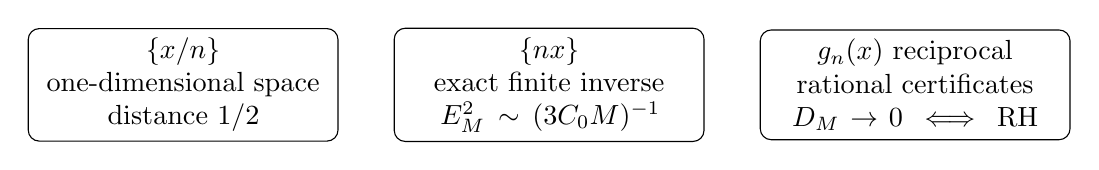
\begin{tikzpicture}[>=Latex,every node/.style={align=center},node distance=9mm]
\node[draw,rounded corners,text width=37mm] (a) {$\{x/n\}$\\one-dimensional space\\distance $1/2$};
\node[draw,rounded corners,text width=37mm,right=7mm of a] (b) {$\{nx\}$\\exact finite inverse\\$E_M^2\sim(3C_0M)^{-1}$};
\node[draw,rounded corners,text width=37mm,right=7mm of b] (c) {$g_n(x)$ reciprocal\\rational certificates\\$D_M\to0\iff\mathrm{RH}$};
\end{tikzpicture}
\caption{The three dictionaries. The ordinary-dilate asymptotic is a
proved approximation theorem. The reciprocal limit is the RH criterion.}
\end{figure}

\section{Rank-one collapse of the linear dictionary}
For $0<x<1$ and $n\ge1$, one has $0<x/n<1$ and therefore
$r_n(x)=x/n$. Every finite span is the line generated by $x$.
Projection of $1$ onto that line gives
\[
 \frac{\langle1,x\rangle}{\langle x,x\rangle}x=\frac32x,
 \qquad
 \left\|1-\frac32x\right\|_2^2
   =1-\frac{(1/2)^2}{1/3}=\frac14.
\]
Thus its distance is $1/2$, independently of $M$.

Writing $d=(1,1/2,\ldots,1/M)^T$, its Gram matrix is
$G^{\rm lin}=dd^T/3$. It has one nonzero eigenvalue $\|d\|^2/3$,
and its Moore--Penrose inverse is
\[
 (G^{\rm lin})^+=\frac{3dd^T}{\|d\|^4}.
\]
Indeed both matrices act by the reciprocal eigenvalues on $\Span(d)$
and vanish on its orthogonal complement. This proves the four
Moore--Penrose identities directly.

\begin{remark}
Increasing the number of coefficients in this dictionary cannot add
directions to the approximation space. A numerical routine returning
different fitted functions at different $M$ is then measuring a
conditioning or implementation effect, not a change in the exact span.
\end{remark}

\section{The ordinary sawtooth Gram matrix}
\subsection{An exact inner product}
Set $v_n=u_n-1/2$. Its mean is zero. The $L^2$ Fourier expansion
of the centered sawtooth is
\[
 \{x\}-\frac12=-\sum_{k\ge1}\frac{\sin(2\pi kx)}{\pi k}.
\]
This follows by integrating against each sine and cosine. Completeness
of the trigonometric system gives the $L^2$ identity; pointwise values
at jumps do not affect an inner product.

\begin{lemma}\label{lem:gcdgram}
For positive integers $j,k$,
\[
 \langle v_j,v_k\rangle=\frac{\gcd(j,k)^2}{12jk},\qquad
 \langle u_j,u_k\rangle=\frac14+\frac{\gcd(j,k)^2}{12jk}.
\]
\end{lemma}
\begin{proof}
Write $j=dj'$, $k=dk'$ with $(j',k')=1$. In the two Fourier
series only matching frequencies contribute. The equation
$\ell j=mk$ requires $\ell=k't$, $m=j't$, $t\ge1$. Orthogonality
therefore gives
\[
 \langle v_j,v_k\rangle
   =\frac1{2\pi^2j'k'}\sum_{t\ge1}\frac1{t^2}
   =\frac1{12j'k'}.
\]
The matching-frequency series is absolutely convergent, justifying
the pairing of the $L^2$ expansions. Adding the product of the means
gives the second formula.
\end{proof}

This formula has no unresolved correction term. For example
$G_{11}=1/3$, $G_{12}=7/24$ and $G_{22}=1/3$.
An independent check in the accompanying program integrates each
piecewise quadratic product over the union of its rational breakpoints.

\subsection{Divisibility factorization}
Let $Z$ be the lower triangular matrix
$Z_{jd}=\boldsymbol1_{d\mid j}$, indexed by $1\le j,d\le M$,
and let $D=\diag(1,2,\ldots,M)$.
The identity $\sum_{d\mid n}J_2(d)=n^2$ follows first for prime
powers by telescoping and then for general $n$ by multiplicativity.
Hence
\begin{equation}\label{eq:factor}
 H_{jk}:=\gcd(j,k)^2,qquad
 H=Z\diag(J_2(1),\ldots,J_2(M))Z^T.
\end{equation}
The inverse of $Z$ has entries
\[
 (Z^{-1})_{jd}=\begin{cases}\mu(j/d),&d\mid j,\\0,&d\nmid j.\end{cases}
\]
Multiplication proves this formula because $\sum_{d\mid n}\mu(d)$
is one for $n=1$ and zero otherwise.

If $C$ is the centered Gram matrix, Lemma~\ref{lem:gcdgram} gives
\begin{align}
 C&=\frac1{12}D^{-1}Z\diag(J_2)Z^TD^{-1},\label{eq:C}\\
 C^{-1}&=12D Z^{-T}\diag(J_2^{-1})Z^{-1}D.\label{eq:Cinverse}
\end{align}
All $J_2(n)$ are positive, so $C$ is positive definite. Moreover
\begin{equation}\label{eq:detC}
 \det C=\frac{\prod_{n\le M}J_2(n)}{12^M(M!)^2}.
\end{equation}
The uncentered matrix is $G=C+\one\one^T/4$, and is also positive
definite. In particular the finite minimizer is unique.

\section{Exact inverse and least-squares solution}
Put $w=C^{-1}\one$ and $A_M=\one^Tw$. Direct multiplication yields
\begin{equation}\label{eq:rankone}
 G^{-1}=C^{-1}-\frac{ww^T}{4+A_M}.
\end{equation}
For completeness, multiplying the right side by $C+\one\one^T/4$
leaves $I$ plus the coefficient
$1/4-1/(4+A_M)-A_M/[4(4+A_M)]=0$ times $\one w^T$.
Thus no matrix-inversion theorem beyond multiplication is required.

Let $q=(1,2,\ldots,M)^T=D\one$. The divisor identity
$\sum_{d\mid n}\mu(n/d)d=\varphi(n)$ gives
$Z^{-1}q=(\varphi(1),\ldots,\varphi(M))^T$. Therefore
\begin{equation}\label{eq:A}
 A_M=12\sum_{n\le M}\frac{\varphi(n)^2}{J_2(n)}=12S_M.
\end{equation}
The $j$th entry of $w$ is
\begin{equation}\label{eq:w}
 w_j=12j\sum_{\substack{k\le M\\j\mid k}}
         \mu(k/j)\frac{\varphi(k)}{J_2(k)}.
\end{equation}

\begin{proof}[Proof of the exact formulas in Theorem~\ref{thm:intro}]
The target vector is $b_j=\langle1,u_j\rangle=1/2$. The normal
equations are $Gc=b=\one/2$. Equations~\eqref{eq:rankone} and
\eqref{eq:A} give
\[
 c=\frac{w}{2(1+3S_M)},
\]
which, by \eqref{eq:w}, is \eqref{eq:exactcoef}. Completing the
quadratic square in
$1-2b^Tc+c^TGc$ gives
\[
 E_M^2=1-b^TG^{-1}b
   =1-\frac{3S_M}{1+3S_M}=\frac1{1+3S_M}.
\]
This also proves optimality directly. The determinant identity
\[
 \det G=\det C\,(1+3S_M)
\]
follows by factoring out $C$ and observing that a rank-one matrix
has only one possibly nonzero eigenvalue.
\end{proof}

For $M=1$, $S_1=1$, $c_1=3/2$ and $E_1^2=1/4$.
For $M=2$, $S_2=4/3$, the coefficients are $(4/5,4/5)$ and
$E_2^2=1/5$. These checks also distinguish this model from the
rank-one family of the preceding section.

\subsection{An arbitrary target}
For real $f\in L^2(0,1)$ put $b_j=\langle f,u_j\rangle$. The unique
coefficient vector is
\[
 c=C^{-1}b-\frac{w(w^Tb)}{4+12S_M},
\]
and the squared error is
\[
 \|f\|_2^2-b^TC^{-1}b+\frac{(w^Tb)^2}{4+12S_M}.
\]
The complex case uses conjugate transposes. Formula~\eqref{eq:Cinverse}
expresses every matrix entry by finite divisor sums. Thus once the
target inner products are known, the optimization requires no
uncontrolled numerical inversion.

\subsection{Arbitrary finite divisor-closed sets}
An initial interval of integers is not essential to the exact inverse.
\begin{theorem}\label{thm:divisorclosed}
Let $\Lambda\subset\N$ be finite, nonempty and closed under taking
positive divisors. Put
$S_\Lambda=\sum_{n\in\Lambda}\varphi(n)^2/J_2(n)$. Then
\[
 \dist\bigl(1,\Span\{u_n:n\in\Lambda\}\bigr)^2
   =\frac1{1+3S_\Lambda}.
\]
The unique minimizing coefficients are
\[
 c_j=\frac{6j}{1+3S_\Lambda}
       \sum_{\substack{k\in\Lambda\\j\mid k}}
           \mu(k/j)\frac{\varphi(k)}{J_2(k)},\qquad j\in\Lambda.
\]
If $\Lambda\subset\Gamma$ are two such sets, the exact improvement
in squared error is
\[
 \frac{3(S_\Gamma-S_\Lambda)}
 {(1+3S_\Lambda)(1+3S_\Gamma)}.
\]
\end{theorem}
\begin{proof}
Order $\Lambda$ increasingly and restrict $D$ and $Z$ to those
indices. Every divisor of a common divisor of two indices remains
in $\Lambda$, so the factorization \eqref{eq:factor} is unchanged.
Every interval of the divisibility order between two members of
$\Lambda$ contains all its integer divisors. Its incidence inverse
is therefore still $\mu(j/d)$ when $d\mid j$. Finally
$Z^{-1}(j)_{j\in\Lambda}=(\varphi(j))_{j\in\Lambda}$ because all
divisors of $j$ are present. The proof of
\eqref{eq:exacterror}--\eqref{eq:exactcoef} now applies verbatim.
Subtracting the two reciprocal error formulas proves the last identity.
\end{proof}

For example $\Lambda=\{1,2,3,6\}$ has $S_\Lambda=2$ and squared
error $1/7$. Such a divisor-closed set need not be an initial interval.
The theorem does not apply to an arbitrary subset without its
divisors: the restricted incidence inverse would then need to be
recalculated.

\section{The asymptotic constant and coefficient decay}
Define $h(n)=\varphi(n)^2/J_2(n)$. At prime powers,
\[
 h(p^k)=\frac{p-1}{p+1}\quad(k\ge1).
\]
Write $h=1*g$ in Dirichlet-convolution notation. Then $g$ is
multiplicative, vanishes on nonsquarefree integers and satisfies
\[
 g(p)=-\frac2{p+1},\qquad |g(n)|\le\frac{\tau(n)}n.
\]
Since $\sum\tau(n)/n^2<\infty$, the series $\sum g(n)/n$ converges
absolutely and equals the Euler product $C_0$ of
\eqref{eq:asymptintro}. Every factor is positive and the sum of their
defects is finite, so $C_0>0$.

\begin{proposition}\label{prop:mean}
For every integer $M\ge1$,
\begin{equation}\label{eq:meanerror}
 |S_M-C_0M|\le(1+\log M)^2+2\log M+4.
\end{equation}
Furthermore $C_0\ge\zeta(2)^{-2}=36/\pi^4$.
\end{proposition}
\begin{proof}
Divisor summation gives
\[
 S_M=\sum_{d\le M}g(d)\lfloor M/d\rfloor.
\]
Replacing the floor by $M/d$ incurs an error at most
\[
 \sum_{d\le M}|g(d)|\le\sum_{d\le M}\frac{\tau(d)}d
 \le\left(\sum_{j\le M}\frac1j\right)^2\le(1+\log M)^2.
\]
For the omitted tail use $T(t)=\sum_{n\le t}\tau(n)\le t(1+\log t)$.
Partial summation and deletion of its nonpositive endpoint term give
\[
 M\sum_{d>M}\frac{\tau(d)}{d^2}
 \le2M\int_M^\infty\frac{1+\log t}{t^2}\,dt
 =2\log M+4.
\]
This proves \eqref{eq:meanerror}. Finally, for each prime $p$,
\[
 1-\frac2{p(p+1)}\ge(1-p^{-2})^2,
\]
as is seen by subtraction. Multiplying finite products and taking
limits proves the stated lower bound.
\end{proof}

The asymptotic in Theorem~\ref{thm:intro} follows immediately.
It is a theorem about ordinary sawtooth approximation, not a
conditional consequence of RH.

\begin{proposition}\label{prop:coefdecay}
Let $H_k=\sum_{j\le k}1/j$. Then
\[
 |c_j^{(M)}|\le\frac{6H_{\lfloor M/j\rfloor}}{1+3S_M},\qquad
 \sum_{j\le M}|c_j^{(M)}|^2\le\frac{180M}{(1+3S_M)^2}.
\]
In particular every fixed coefficient tends to zero and the squared
coefficient norm is $O(M^{-1})$.
\end{proposition}
\begin{proof}
The prime-power formula gives $\varphi(k)/J_2(k)\le1/k$.
Taking absolute values in \eqref{eq:exactcoef} yields the first bound.
Since $H_{\lfloor M/j\rfloor}\le1+\log(M/j)$ and the latter squared
is decreasing in $j$,
\[
 \sum_{j=1}^M(1+\log(M/j))^2
 \le\int_0^M(1+\log(M/x))^2\,dx=5M.
\]
The second bound follows. Proposition~\ref{prop:mean} supplies the
asymptotic conclusions.
\end{proof}

Thus the least-squares coefficients in this problem do not converge
termwise to $\mu(j)$. The M\"obius function enters the inverse of the
divisibility matrix; its appearance there is not a termwise coefficient
limit.

\begin{figure}[tb]
\centering
\begin{tikzpicture}
\begin{axis}[width=.84\textwidth,height=5cm,xlabel={$M$},ylabel={$E_M^2$},
 xmode=log,ymode=log,grid=major,legend style={at={(.98,.98)},anchor=north east}]
\addplot[blue!70!black,thick,mark=*,mark size=1.4pt] table[x=M,y=error,col sep=comma]{ordinary.csv};
\addlegendentry{exact finite formula}
\addplot[orange!80!black,dashed,thick] table[x=M,y=comparison,col sep=comma]{ordinary.csv};
\addlegendentry{$1/(3C_{100000}M)$}
\end{axis}
\end{tikzpicture}
\caption{Finite errors from exact rational $S_M$. The comparison uses
the explicitly truncated prime product $C_{100000}$, not an asserted
decimal value for the infinite product. All plotted values are regenerated
by the accompanying checker.}
\end{figure}

\section{Mellin transforms with the correct dictionary}
For $f$ on $(0,1)$ write
$\mathcal Mf(s)=\int_0^1 f(x)x^{s-1}\,dx$ wherever the integral exists.
The elementary identity
\[
 \{nx\}=nx-\sum_{j=1}^{n-1}\boldsymbol1_{[j/n,1)}(x)
\]
gives, for $\Re s>0$,
\begin{equation}\label{eq:ordinarymellin}
 \mathcal Mu_n(s)=\frac n{s+1}-\frac{n-1}s
                  +\frac{n^{-s}}s\sum_{j=1}^{n-1}j^s.
\end{equation}
There is no zeta factor in this finite expression. Apparent singularities
at zero are removable whenever the original integral continues there.

For the reciprocal functions let $0<\theta\le1$. When $\Re s>1$,
expand the floor into nonnegative indicator functions and integrate:
\begin{align*}
 \int_0^1\{\theta/x\}x^{s-1}\,dx
 &=\theta\int_0^1x^{s-2}\,dx
       -\sum_{k\ge1}\int_0^{\theta/k}x^{s-1}\,dx\\
 &=\frac\theta{s-1}-\frac{\theta^s\zeta(s)}s.
\end{align*}
For complex $s$ absolute convergence justifies the sum; it follows
first on the real axis and then analytically. The left side is analytic
on $\Re s>0$, since the fractional part is bounded. The right side
has a removable singularity at $s=1$ and agrees there by continuation.
Consequently
\begin{equation}\label{eq:reciprocalmellin}
 \mathcal Mg_n(s)=-\frac{\zeta(s)}s(n^{-s}-n^{-1}),\qquad \Re s>0.
\end{equation}
At $s=1$, the zero of $n^{-s}-n^{-1}$ cancels the pole of $\zeta$,
and
\begin{equation}\label{eq:bn}
 b_n:=\langle1,g_n\rangle=\frac{\log n}{n}.
\end{equation}

\subsection{Why the centered criterion is the right one}
The strong B\'aez-Duarte criterion is stated in $L^2(0,\infty)$ using
$\rho_n(x)=\{1/(nx)\}$ and target $\boldsymbol1_{(0,1)}$
\cite{BD}. For $x>1$, $\rho_n(x)=1/(nx)$. If
$f=\sum_{n\le M}a_n\rho_n$ and $A=\sum a_n/n$, then its squared
tail norm on $(1,\infty)$ is $A^2$. Also $\rho_1\in L^2(0,\infty)$.
Thus any approximating sequence with error tending to zero has $A\to0$,
and replacing $f$ by $f-A\rho_1$ changes its norm by at most
$|A|\|\rho_1\|_2\to0$. The replacement equals
$\sum_{n=2}^M a_n(\rho_n-n^{-1}\rho_1)$ and vanishes for $x>1$.
Conversely such centered approximants extend by zero and already lie
in the original integer-dilate span. This proves equivalence between
the cited criterion and \eqref{eq:RHcriterion}.

\section{Rational certificates for the reciprocal Gram matrix}
\subsection{Step values and a positive series}
Let $q=\lfloor1/x\rfloor$, so $1/x=q+t$ with $0\le t<1$. For any
integer $n\ge2$,
\[
 \lfloor(q+t)/n\rfloor=\lfloor q/n\rfloor.
\]
Substitution in \eqref{eq:gn} gives the exact step-function identity
\begin{equation}\label{eq:step}
 g_n(x)=\{q/n\}\quad\text{for }\frac1{q+1}<x\le\frac1q.
\end{equation}
Boundary conventions affect a null set only.

Let $v_q=(\{q/2\},\ldots,\{q/M\})^T$ and
$w_q=1/[q(q+1)]$. The reciprocal Gram matrix is
\begin{equation}\label{eq:Bseries}
 B=\sum_{q\ge1}w_qv_qv_q^T,qquad
 B^{(Q)}=\sum_{q=1}^Qw_qv_qv_q^T.
\end{equation}
Every truncated matrix is rational and positive semidefinite. The
tail is positive semidefinite as well. Entrywise,
\begin{equation}\label{eq:tailentry}
 0\le B_{nm}-B^{(Q)}_{nm}\le\sum_{q>Q}w_q=\frac1{Q+1}.
\end{equation}
For a real vector $c$, its quadratic tail obeys
\begin{equation}\label{eq:tailquad}
 0\le c^T(B-B^{(Q)})c\le\frac{\|c\|_1^2}{Q+1}.
\end{equation}
The lower bound uses positive semidefiniteness, not entrywise
positivity with arbitrary signed coefficients. This distinction is
important when using optimized vectors.

\subsection{A finite determinant certificate}
\begin{theorem}\label{thm:reciprocaldet}
For $M\ge2$, let $V$ have rows $q=1,\ldots,M-1$ and columns
$n=2,\ldots,M$, with $V_{qn}=\{q/n\}$. Then
\[
 |\det V|=\frac1M,\qquad
 \det B^{(M-1)}=\frac1{M(M!)^2}.
\]
In particular $B^{(Q)}$ is positive definite for every $Q\ge M-1$,
and so is $B$.
\end{theorem}
\begin{proof}
Retain the first row. For $q\ge2$, replace row $q$ by its difference
with row $q-1$, performing these operations in descending order.
The new entry is $1/n-\boldsymbol1_{n\mid q}$. Subtract the first
row, whose entries are $1/n$, from each of these rows. The resulting
lower rows have entries $-\boldsymbol1_{n\mid q}$. Their block with
$2\le q,n\le M-1$ is lower triangular with diagonal $-1$.
The final column $n=M$ vanishes in every lower row and has first
entry $1/M$. Expansion along this column proves the first identity.

Since $B^{(M-1)}=V^T\diag(w_1,\ldots,w_{M-1})V$,
\[
 \det B^{(M-1)}=\frac1{M^2}\prod_{q=1}^{M-1}\frac1{q(q+1)}
   =\frac1{M(M!)^2}.
\]
All diagonal weights are positive and $V$ is nonsingular. Adding
further positive semidefinite terms preserves positive definiteness.
\end{proof}

A crude but completely explicit lower eigenvalue certificate follows.
Put $N=M-1$. Since the diagonal entries of $B^{(M-1)}$ are at most
one, its trace is at most $N$. All eigenvalues are positive, and
the product of the $N-1$ largest is at most $N^{N-1}$. Hence
\begin{equation}\label{eq:lambda}
 \lambda_{\min}(B)\ge\lambda_{\min}(B^{(M-1)})
 \ge\frac1{M(M!)^2N^{N-1}}.
\end{equation}
For $N=1$ the power $N^0$ is one. The bound is conservative, but
requires neither floating-point diagonalization nor a conjecture.

\subsection{Certified residual intervals}
For any rational vector $c=(c_2,\ldots,c_M)$ define
\[
 R(c)=\left\|1-\sum_{n=2}^M c_ng_n\right\|_2^2.
\]
Equations~\eqref{eq:bn} and \eqref{eq:Bseries} give
\begin{equation}\label{eq:residual}
 R(c)=1-2\sum_{n=2}^M\frac{c_n\log n}{n}
             +\sum_{q\ge1}\frac{(c^Tv_q)^2}{q(q+1)}.
\end{equation}
Suppose rational intervals $L_n\le\log n\le U_n$ have been proved.
Taking sign-aware interval bounds in the finite linear sum and using
\eqref{eq:tailquad} then gives a rigorous interval for $R(c)$.
The checker uses the positive series
\begin{equation}\label{eq:logseries}
 \log x=2\sum_{k\ge0}\frac{t^{2k+1}}{2k+1},\qquad
 t=\frac{x-1}{x+1},\quad x\ge1.
\end{equation}
After $K$ terms the omitted tail is between zero and
$2t^{2K+1}/[(2K+1)(1-t^2)]$. Thus all endpoints can be rational.
Range reduction by powers of two keeps this certificate efficient.

These intervals certify individual finite residuals, and therefore
upper bounds for $D_M^2$.\footnote{A finite upper bound is a proved
inequality for chosen coefficients. Convergence to zero requires a
uniform analytic estimate for a sequence of residuals.}
They do not certify that an unspecified
sequence of residuals tends to zero. The determinant theorem proves
finite independence, not the density assertion in
\eqref{eq:RHcriterion}.

\section{The Mellin Hardy space and zero obstructions}
\subsection{The correct reproducing kernel}
For $f\in L^2(0,1)$ set $F(s)=\mathcal Mf(s)$ on $\Re s>1/2$.
Cauchy--Schwarz gives
\begin{equation}\label{eq:evaluation}
 |F(s)|\le\frac{\|f\|_2}{\sqrt{2\Re s-1}}.
\end{equation}
The kernel is
\begin{equation}\label{eq:kernel}
 K(s,w)=\int_0^1x^{s+\overline w-2}\,dx
       =\frac1{s+\overline w-1}.
\end{equation}
Under $x=e^{-t}$ and $h(t)=e^{-t/2}f(e^{-t})$,
\[
 F(1/2+z)=\int_0^\infty h(t)e^{-zt}\,dt,\qquad
 \|h\|_{L^2(0,\infty)}=\|f\|_2.
\]
Plancherel on vertical lines therefore gives the Hardy norm identity
\[
 \sup_{\sigma>1/2}\frac1{2\pi}\int_{\R}|F(\sigma+it)|^2dt
       =\|f\|_2^2.
\]
The supremum is the limit as $\sigma\downarrow1/2$, by monotone
convergence applied to $|h(t)|^2e^{-2(\sigma-1/2)t}$.
These formulas describe the Mellin image as a reproducing-kernel
Hilbert space; the usual Laplace-transform Hardy-space theorem
identifies it with $H^2(\Re s>1/2)$. The norm and evaluations used here
already follow from the displayed calculation.

Boundary point evaluation is not bounded. For fixed $t_0\in\R$, let
\[
 f_N(x)=\frac{x^{-1/2-it_0}}{\sqrt N}
              \boldsymbol1_{[e^{-N},1]}(x).
\]
Then $\|f_N\|_2=1$ but
$\mathcal Mf_N(1/2+it_0)=\sqrt N$.
Hence \eqref{eq:evaluation} cannot be extended to a uniform pointwise
bound on the critical line. A boundary $L^2$ norm is a different
statement from bounded evaluation at one boundary point.

\subsection{Bounds conditional on off-line zeros}
\begin{proposition}\label{prop:zerobound}
If $\zeta(\rho)=0$ and $\beta=\Re\rho>1/2$, then for every $M$,
\[
 D_M^2\ge\frac{2\beta-1}{|\rho|^2}.
\]
More generally, for distinct such zeros $\rho_1,\ldots,\rho_k$, put
$K_{ij}=1/(\rho_i+\overline{\rho_j}-1)$ and $v_i=1/\rho_i$.
Then $D_M^2\ge v^*K^{-1}v$.
\end{proposition}
\begin{proof}
For any residual $f=1-\sum c_ng_n$, its Mellin transform is
\[
 F(s)=\frac1s+\frac{\zeta(s)}s\sum_{n=2}^M c_n(n^{-s}-n^{-1}).
\]
Thus $F(\rho)=1/\rho$. Applying \eqref{eq:evaluation} proves the
single-zero bound and taking the infimum over $c$ preserves it.

For several zeros, the evaluation representers have Gram matrix $K$.
They are linearly independent: a vanishing linear combination of
their kernels would be a rational function with distinct poles and
therefore have every coefficient zero. The least norm interpolant
with evaluation vector $v$ has squared norm $v^*K^{-1}v$, as follows
by projecting onto their span and solving its finite Gram system.
Every residual has those evaluations, so its norm is at least that
quantity. This proves the second assertion.
\end{proof}

The proposition neither asserts an off-line zero nor excludes one.
It gives a rigorous obstruction if such a zero is supplied. In
particular it provides no missing upper bound that would force
$D_M\to0$.

\section{Filtering a sequence of finite approximation errors}
The previous version introduced a Kalman filter for noisy evaluations
of approximation errors. Such filtering is an estimation problem;
it cannot establish an unproved limit of the exact sequence. We give
the corrected finite formulas, with assumptions stated explicitly.

\subsection{Fixed gain}
Let $0<K\le1$, $r=1-K$, and suppose observations are
$z_m=d_m+\varepsilon_m$. Define
\[
 \widehat d_m=r\widehat d_{m-1}+Kz_m,qquad
 e_m=\widehat d_m-d_m.
\]
For deterministic $d_m$ and deterministic starting value,
\begin{equation}\label{eq:filtererror}
 e_m=r^me_0+r\sum_{j=1}^m r^{m-j}(d_{j-1}-d_j)
                   +K\sum_{j=1}^m r^{m-j}\varepsilon_j.
\end{equation}
This follows by substituting the recursion and iterating it; $d_0$
is the target value associated with the initial estimate.

Assume the noises are independent, centered and sub-Gaussian with
variance proxy $\sigma^2$, meaning
$\E e^{t\varepsilon_j}\le e^{\sigma^2t^2/2}$ for all real $t$.
Independence and multiplication of moment-generating functions show
that the final sum in \eqref{eq:filtererror} is sub-Gaussian with proxy
\begin{equation}\label{eq:variancefloor}
 \sigma^2K^2\sum_{j=0}^{m-1}r^{2j}
 =\frac{\sigma^2K}{2-K}(1-r^{2m}).
\end{equation}
If the target is constant and the noises are independent with actual
variance $\sigma^2>0$, the variance tends to
$\sigma^2K/(2-K)>0$. Thus a fixed positive gain does not yield
vanishing mean-square error in this model.

If $|d_j-d_{j-1}|\le\Delta$, its deterministic bias satisfies
\[
 |\E e_m|\le r^m|e_0|+\frac{r\Delta(1-r^m)}K.
\]
Combining this with \eqref{eq:variancefloor} gives a complete
finite mean-square and tail estimate. For example, with probability
at least $1-\delta$, the absolute stochastic part is at most
$\sqrt{2\sigma^2K(1-r^{2m})\log(2/\delta)/(2-K)}$.

\subsection{The random-walk gain and a vanishing-gain alternative}
In the scalar random-walk model with process variance $Q>0$ and
observation variance $R>0$, a steady posterior variance $P$ satisfies
\[
 K=\frac{P+Q}{P+Q+R},\qquad P=R K.
\]
Eliminating $P$ yields $RK^2+QK-Q=0$. Its unique root in $(0,1)$ is
\begin{equation}\label{eq:gain}
 K=\frac{\sqrt{Q^2+4QR}-Q}{2R}.
\end{equation}
The underlying filtering framework is due to Kalman \cite{Kalman};
the scalar algebra above is included to fix the normalization.

If instead the gain is $1/m$, induction gives
$\widehat d_m=m^{-1}\sum_{j=1}^m z_j$. Under the same independent
noise assumption, its variance is at most $\sigma^2/m$. If the target
sequence satisfies the independently established estimate
$|d_j-d|\le Cj^{-\alpha}$, then
\[
 |\E\widehat d_m-d|\le\frac C m\sum_{j=1}^m j^{-\alpha}.
\]
This is $O(m^{-\alpha})$ for $0<\alpha<1$, $O(\log m/m)$ for
$\alpha=1$, and $O(m^{-1})$ for $\alpha>1$. The assumption on the
exact target sequence is indispensable. Applying a filter to numerical
values of $D_M$ does not prove that assumption or RH.

\begin{figure}[tb]
\centering
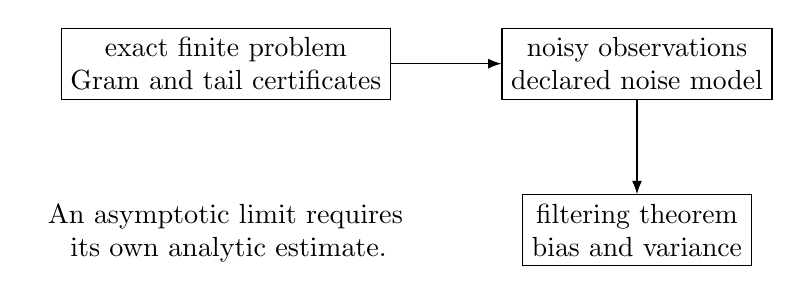
\begin{tikzpicture}[>=Latex,node distance=10mm,every node/.style={align=center}]
\node[draw] (exact) {exact finite problem\\Gram and tail certificates};
\node[draw,right=14mm of exact] (obs) {noisy observations\\declared noise model};
\node[draw,below=12mm of obs] (filter) {filtering theorem\\bias and variance};
\draw[->] (exact)--(obs);\draw[->] (obs)--(filter);
\node[below=12mm of exact,text width=48mm] {An asymptotic limit requires its own analytic estimate.};
\end{tikzpicture}
\caption{Exact approximation and statistical estimation have different
inputs. A filter controls observation error under a noise model.}
\end{figure}

\section{Exact verification and limits of the results}
The standard-library program \texttt{checks/verify.py} performs exact
rational integration of ordinary sawtooth products, checks the GCD
formula, verifies the divisor factorization and the normal equations,
and compares the exact optimum with \eqref{eq:exacterror}. It also
checks the reciprocal step matrix and determinant for a finite range
of $M$, constructs certified logarithm intervals, and bounds selected
rational residuals by \eqref{eq:residual}.

These finite checks support the stated identities but do not replace
their proofs for arbitrary $M$. The graph uses only values generated
from the proved ordinary-dilate formula. No synthetic experimental
dataset, numerical zero exclusion or full proof-assistant audit is
claimed.

The ordinary problem is solved exactly and unconditionally. The
reciprocal problem has finite positive-definiteness and rigorous
residual certificates, but the limit in \eqref{eq:RHcriterion} remains
unproved. Classical identities and cited RH criteria are credited;
the present calculations are not presented as a resolution of RH or
as a certified new major conjecture closure.

\appendix
\section{A direct rational integration algorithm}
To integrate $u_j u_k$, sort the finite set
\[
 \{0,1\}\cup\{a/j:1\le a<j\}\cup\{b/k:1\le b<k\}.
\]
On an open interval $(\alpha,\beta)$ in this partition, the floor
values $A=\lfloor jx\rfloor$ and $B=\lfloor kx\rfloor$ are constant.
The product is $jkx^2-(jB+kA)x+AB$, so the integral is exactly
\[
 \frac{jk}{3}(\beta^3-\alpha^3)
 -\frac{jB+kA}{2}(\beta^2-\alpha^2)+AB(\beta-\alpha).
\]
All terms are rational. This gives an independent finite computation
of Lemma~\ref{lem:gcdgram}, with no Fourier truncation or quadrature.

\section{Determinants, optimization and conditioning}
For any real positive-definite Gram matrix $A$ and target vector $b$,
\[
 \|f-\textstyle\sum c_ju_j\|^2
 =\|f\|^2-b^TA^{-1}b+(c-A^{-1}b)^TA(c-A^{-1}b).
\]
This identity proves uniqueness of the minimizer and its exact error.
It does not require estimating a condition number.
When a floating-point approximation $\widetilde c$ is used instead,
the excess squared error is exactly
$(\widetilde c-c)^TA(\widetilde c-c)$.

For the reciprocal matrix, the positive tail in \eqref{eq:Bseries}
shows $B\succeq B^{(Q)}$ in Loewner order. Entrywise error bounds
alone would not imply that ordering. Conversely the tail's operator
norm is at most its trace, hence at most $(M-1)/(Q+1)$.
If $B^{(Q)}$ has a certified lower eigenvalue $\lambda>0$, then
\[
 \|(B^{(Q)})^{-1}-B^{-1}\|
 \le\frac{M-1}{\lambda^2(Q+1)},
\]
by the resolvent identity and $\|B^{-1}\|\le1/\lambda$.
This is a finite error estimate, not an asymptotic density theorem.

\section{A rational logarithm certificate}
For $x\ge1$, write $t=(x-1)/(x+1)$. The identity
$\log x=\log(1+t)-\log(1-t)$ follows by solving for $x$.
Integrating the geometric series for $2/(1-t^2)$ proves
\eqref{eq:logseries}. After $K$ terms,
\[
 0\le\log x-2\sum_{k=0}^{K-1}\frac{t^{2k+1}}{2k+1}
 \le\frac{2t^{2K+1}}{(2K+1)(1-t^2)}.
\]
For an integer $n$, choose $a$ with $1\le n/2^a<2$. Apply the
formula to $2$ and to $n/2^a$; then use
$\log n=a\log2+\log(n/2^a)$. All quantities in the finite sums and
tail bounds are rational. The terms have $0\le t\le1/3$, so the
tail decreases geometrically. For a signed coefficient $c_n$, the
lower and upper logarithm endpoints must be interchanged when the
coefficient multiplying the logarithm is negative.

\section{Revision record}
The prior version \cite{Previous} discussed rank-one collapse,
sawtooth inner products, Mellin transforms, Hardy bounds and filtering.
All five topics are retained, but their mathematical relations have
been corrected. The ordinary Gram formula is exact; its inverse,
least-squares coefficients and mean constant are derived. Reciprocal
functions now have separate notation, a proved step representation,
a finite determinant certificate and a rational tail bound.

The previous zeta-dependent kernel and critical-line pointwise bound
are replaced by \eqref{eq:kernel} and the explicit boundary
counterexample. The fixed-gain decay claim is replaced by the exact
variance floor, and the scalar Riccati root is corrected. Claims
depending on unverified numerical data or an unproved limiting
estimate have been removed. The stronger title refers to the fully
derived finite inverse, not a claimed solution of RH.

\section*{Declarations and availability}
\textbf{Competing interests.} The authors declare no competing interests.
\textbf{Funding.} No specific funding is reported in the supplied source.
\textbf{Ethics.} The work uses no human participants or animals.
\textbf{Authorship.} The author order and corresponding author of the
published version are preserved. Affiliations are reproduced from the
supplied sources; Pallab Nandi's IISER association is historical.
\textbf{Computational and editorial assistance.} AI assistance was used
for source review, derivation checks, code and preparation of this
revision. It is not an author. The provenance file distinguishes the
analytic proofs from the finite computational checks. No Lean
formalization is claimed.
\textbf{Acknowledgements.} The presentation builds on the work of
Nyman, Beurling, B\'aez-Duarte, Smith and Kalman, and on the cited GCD
sum literature. No endorsement by these researchers is implied.
\par\textbf{Repository and release.} \url{https://github.com/creelie/nyman-beurling-approximation}. Release \href{https://github.com/creelie/nyman-beurling-approximation/releases/tag/v3.0.1}{v3.0.1}.
\par\textbf{Permanent work DOI.} \href{https://doi.org/10.5281/zenodo.24054093}{10.5281/zenodo.24054093}. This DOI identifies the work across archived releases; the version-specific DOI is recorded on the linked archive page.


\begin{thebibliography}{9}
\bibitem{Smith} H. J. S. Smith, On the value of a certain arithmetical
determinant, \emph{Proc. London Math. Soc.} \textbf{s1-7} (1875), 208--213.
\href{https://doi.org/10.1112/plms/s1-7.1.208}{doi:10.1112/plms/s1-7.1.208}.
\bibitem{ABS} C. Aistleitner, I. Berkes and K. Seip, GCD sums from
Poisson integrals and systems of dilated functions,
\emph{J. Eur. Math. Soc.} \textbf{17} (2015), 1517--1546.
\href{https://doi.org/10.4171/JEMS/537}{doi:10.4171/JEMS/537}.
\bibitem{Beurling} A. Beurling, A closure problem related to the Riemann
zeta-function, \emph{Proc. Natl. Acad. Sci. USA} \textbf{41} (1955), 312--314.
\href{https://doi.org/10.1073/pnas.41.5.312}{doi:10.1073/pnas.41.5.312}.
\bibitem{BD} L. B\'aez-Duarte, A strengthening of the Nyman--Beurling
criterion for the Riemann hypothesis, \emph{Atti Accad. Naz. Lincei Rend.
Lincei Mat. Appl.} (9) \textbf{14} (2003), 5--11.
\url{https://www.bdim.eu/item?id=RLIN_2003_9_14_1_5_0}.
\bibitem{Kalman} R. E. Kalman, A new approach to linear filtering and
prediction problems, \emph{J. Basic Eng.} \textbf{82} (1960), 35--45.
\href{https://doi.org/10.1115/1.3662552}{doi:10.1115/1.3662552}.
\bibitem{Previous} D. Bhattacharjee, P. Nandi, O. Frederick and
P. Samal, Spectral and analytic structure of the Nyman--Beurling--B\'aez--Duarte
approximation, \emph{Preprints.org} (2026), 202506.0772, version 2.
\url{https://www.preprints.org/manuscript/202506.0772/v2}.
\end{thebibliography}
\end{document}
